% Chapter 7

\chapter{Topology and symmetries} % Main chapter title

\label{Chapter7} % For referencing the chapter elsewhere, use \ref{Chapter7} 

\lhead{Part II. \emph{One wire}}
\chead{Chapter 7. \emph{Topology \& symmetries}} % This is for the header on each page - perhaps a shortened title

%----------------------------------------------------------------------------------------
In this chapter we will define the socalled time reversal and particle-hole transformations. This we will use to come with a topological characterization of the now developed Kitaev model system. It entails defining a topological index $\nu$, that describes whether the system is in a topological or trivial phase. Finally, we will see what physical consequences the phases have by discussing the bulk-edge correspondence principle and edge states. The treatment is heavily based on the articles \cite{Ludwig.Topology, Chiu.Topology, Alicea}. 

\section{The time reversal and particle-hole transformations and symmetries}
\label{sec.SymmetriesTRandPH}
In this section we define the time reversal and particle-hole transformations. Let us remind ourselves of the form of the noninteracting Hamiltonian obtained after the mean field approximation of chapter \ref{Chapter4}: 
\begin{equation}
H_{FF} = -\sum_k \Delta_k \braket {c^\dagger_k c^\dagger_{-k}} + \frac{1}{2}\sum_{k} \begin{bmatrix} c^\dagger_k & c_{-k} \end{bmatrix} \begin{bmatrix} \varepsilon_k & \Delta_k \\ \Delta^*_k & -\varepsilon_k \end{bmatrix} \begin{bmatrix} c_k \\ c^\dagger_{-k} \end{bmatrix}. \nonumber 
\end{equation}

It is clear, that the Hamiltonian is translationally invariant. Explicitly, the (unitary) translation operator is defined through: $\tau(x_0)\psi_F(x)\tau^\dagger (x_0) = \psi_F(x+x_0)$. In momentum space, we hereby get $\tau(x_0) c_k \tau^\dagger(x_0) = \text{e}^{ikx_0}c_k$, as one might expect. Hence, terms like $c^\dagger_k c_k, c_k c^\dagger_k, c^\dagger_kc^\dagger_{-k}$ and $c_{-k}c_k$ are invariant under the translation. This means, that $H_{FF}$ is invariant as well. Because of the translational invariance, we \textit{inforce} that the time reversal and particle-hole transformations do not mix states with different positions. Specifically:
\begin{align}
T \begin{bmatrix} \psi_F(x) \\ \psi^\dagger_F(x) \end{bmatrix} T^{-1} &= U^\dagger_T \begin{bmatrix} \psi_F(x) \\ \psi^\dagger_F(x) \end{bmatrix}, \hspace{0.5cm} TiT^{-1} = -i, \nonumber \\
C \begin{bmatrix} \psi_F(x) \\ \psi^\dagger_F(x) \end{bmatrix} C^{-1} &= (U^*_C)^\dagger \begin{bmatrix} \psi^\dagger_F(x) \\ \psi_F(x) \end{bmatrix}, \hspace{0.5cm} CiC^{-1} = i.  
\label{eq.TRandPH.realspace}
\end{align}
Here $T$ and $C$ is the time reversal and particle-hole transformation respectively. $U_T$ and $U_C$ are $2\times 2$ matrices. Inforcing that transformed operators are fermionic as well, means that the matrices have to be unitary. The operation on $i$ specifies, that $T$ is antiunitary and $C$ is unitary. In momentum space this definition leads to:
\begin{align}
T \begin{bmatrix} c_k \\ c^\dagger_{-k} \end{bmatrix} T^{-1} &= U^\dagger_T \begin{bmatrix} c_{-k} \\ c^\dagger_{k} \end{bmatrix}, \nonumber \\
C \begin{bmatrix} c_k \\ c^\dagger_{-k} \end{bmatrix} C^{-1} &= (U^*_C)^\dagger \begin{bmatrix} c^\dagger_{-k} \\ c_{k} \end{bmatrix}. 
\label{eq.TRandPH.momentumspace}
\end{align}
By inspecting the transformations $TH_{FF}T^{-1}$ and $CH_{FF}C^{-1}$, we get the following symmetry requirements:
\begin{align}
TH_{FF}T^{-1} = H_{FF} \Leftrightarrow U_T\mathcal{H}^*_{FF,-k} U^\dagger_T = + \mathcal{H}_{FF,+k}, \nonumber \\
CH_{FF}T^{-1} = H_{FF} \Leftrightarrow U_C\mathcal{H}^*_{FF,-k} U^\dagger_C = - \mathcal{H}_{FF,+k}. 
\label{eq.Symmetryrequirements}
\end{align}
This means, that we can think of the second quantization transformations $T$ and $C$ in terms of first quantization antiunitary transformations $\mathcal{T} = U_TK, \mathcal{C} = U_CK$, where $K$ is the complex conjugation operator. This is a general property of these transformation, not restricted to our specific system. See e.g. the articles \cite{Ludwig.Topology, Chiu.Topology}. The Hamiltonian at hand is a socalled Bogoliubov-de Gennes (BdG) Hamiltonian. These BdG Hamiltonians in general has a particle-hole symmetry. The reason is, that there is a redundancy in the matrix structure of the Hamiltonian. Explicitly, the structure contains a $2\times 2$ matrix, even though there is only one energy solution. Another way of putting this, is that the two Nambu spinors on each side of the kernel $\mathcal{H}_{FF,k}$ are not independent. We can transform one into the other by going to $-k$ and flipping the entries. The redundancy is here especially evident, since we can simply choose $C$ to have no effect on the Nambu spinor:
\begin{equation}
C \begin{bmatrix} c_k \\ c^\dagger_{-k} \end{bmatrix} C^{-1} =  \sigma_1 \begin{bmatrix} c^\dagger_{-k} \\ c_{k} \end{bmatrix} = \begin{bmatrix} c_k \\ c^\dagger_{-k} \end{bmatrix}, 
\end{equation}
with $\sigma_1$ the first Pauli matrix. This of course means, that $H_{FF}$ is invariant under $C$. Since, it stems from a redundancy in the \textit{structure} of the Hamiltonian, it is often referred to as a particle-hole \textit{constraint} of BdG systems rather than a symmetry. This also means, that for the system to be consistent, we need $\sigma_1\mathcal{H}^*_{FF,+k} \sigma_1 = - \mathcal{H}_{FF,-k}$, which can also explicitly be checked. 

The time reversal case is somewhat trickier. Firstly, in general the pairing $\Delta_k$ is complex. However, as seen in the previous chapters we can explicitly find a real solution. This is also evident mathematically. For this purpose we let $\Delta_k \to \text{e}^{i\phi}\Delta_k$, with $\phi$ the phase of the pairing, and now $\Delta_k$ real. We then perform a gauge transformation in the $c_k$ operators according to: $c_k \to \text{e}^{-i\phi/2} c_k$. Since $\Delta_k$ depends linearly on $\braket{c_kc_{-k}}$ the resulting transformation of the pairing is:
\begin{equation}
\text{e}^{i\phi}\Delta_k \to \text{e}^{i\phi}\Delta_k\text{e}^{-i\phi} = \Delta_k. \nonumber
\end{equation}
With this the kernel $\mathcal{H}_{FF,k}$ is real, and with $U_T = i\sigma_3$ we get a time reversal symmetry in accordance with equation \ref{eq.Symmetryrequirements}. Explicitly:
\begin{equation}
U_T\mathcal{H}^*_{FF,-k}U^\dagger_T = \sigma_3\mathcal{H}^*_{FF,-k}\sigma_3 = \begin{bmatrix} 1 & 0 \\ 0 & -1 \end{bmatrix}\begin{bmatrix} \varepsilon_k & -\Delta_k \\ -\Delta_k & -\varepsilon_k \end{bmatrix} \begin{bmatrix} 1 & 0 \\ 0 & -1 \end{bmatrix} = \begin{bmatrix} \varepsilon_k & \Delta_k \\ \Delta_k & -\varepsilon_k \end{bmatrix} = \mathcal{H}_{FF,k}, \nonumber
\end{equation}
since $\Delta_k$ is odd in k and now also real. It is evident, that the found time reversal symmetry physically transforms a particle into a particle with opposite momentum:
\begin{equation}
T \begin{bmatrix} c_k \\ c^\dagger_{-k} \end{bmatrix} T^{-1} = \begin{bmatrix} i c_{-k} \\ - i c^\dagger_{k} \end{bmatrix}. \nonumber
\end{equation}
It is intuitively reasonable, that this \textit{should} be a symmetry of the system. Physically the fermions are bound in Cooper pairs of momentum $k$ and $-k$. This time reversal transformation transforms such a pair by flipping the momentum of both fermions. However, this is still a Cooper pair of momentum $k$ and $-k$. This also emphasizes the fact, that this time reversal symmetry is present due to a unitary parity symmetry. 

\section{Sublattice transformation and topological classification}
By composing the time reversal and particle-hole transformations we can form a third transformation: the socalled sublattice (or chiral) symmetry $S = TC$. It is evident, that this transformation is antiunitary like $T$. The same analysis as in the previous section leads to the symmetry condition:
\begin{equation}
SH_{FF}S^{-1} = H_{FF} \Leftrightarrow U_S\mathcal{H}_{FF,-k} U^\dagger_S = - \mathcal{H}_{FF,+k}.
\end{equation}
Hence, the transformation in first quantization is unitary, but has to anticommute with the Hamiltonian. It is also evident, that since the system at hand both has a time reversal and particle-hole symmetry, we can simply form the product to get the symmetry with $U_S = \sigma_3\sigma_1 = i\sigma_2$, $\sigma_j$ being the Pauli matrices. The reason for including this third transformation is the following. 

In the articles \cite{Ludwig.Topology, Chiu.Topology} it is studied, how one can classify all noninteracting fermionic Hamiltonians, that has an energy gap in the spectrum. The result is, that one needs three and only three transformations: time reversal, particle-hole and sublattice. Further there are three distinct possibilities for the two first. Either there is no symmetry or there is a symmetry and then the transformations can square to $\pm \mathbb{I}$. The sublattice transformation can only be realised in one way, yielding in total two possibilites. Further, as the system at hand explicitly shows, if there is both a time reversal, $T$, and particle-hole symmetry, $C$ there is also a sublattice symmetry, $S$. Further, if only $T$ or $C$ is present of the two, there cannot be a sublattice symmetry. Else, we would be able to make the remaining symmetry by composition. However, in the case of no $T$ nor $C$ symmetry, there is still two possibilities for $S$: symmetry or no symmetry. This is the reason why this last symmetry is included. This yields $(3\cdot 3 - 1) + 2 = 10$ possibilities of combining the symmetries. It is therefore also referred to as the 10-fold way. The first remarkable thing, which I have not argued for, is that this classification is complete. There is nothing else to learn from the topology of the system. 

The second remarkable thing, which I will not argue for either, is that the classification puts the Hamiltonian in a specific Cartan class. The information from the classification is, that the socalled topological index has to be found in a specific set of numbers. This set can for example be the integers $\mathbb{Z}$. The result of the articles is then, that if two ground states have different integers as their topological index, they cannot be deformed continously into each other without closing the energy gap. The socalled periodic table for topological insulators and superconductors is shown in table \ref{tab.PeriodicTableTISC}.

\begin{table}[htb]
\centering
\caption{\textit{Periodic table of topological superconductors and insulators. $d$ is the spatial dimension. A 0-value for T,C and S indicates no symmetry. For T and C the sign indicates the sign of the square $T^2$ and $C^2$ for a symmetry present. $S=1$ indicates presence of a sublattice symmetry. The sets to the right indicates in what set of numbers the topological index should be found. }}
\begin{tabular}{|l|l l l|l l l l|}
\hline Cartan/$d$   &  T &  C & S					& 0 & 1 & 2 & 3 \\
\hline A    		&  0 &  0 & 0					& $\mathbb{Z}$ & 0 & $\mathbb{Z}$ & 0   			 \\
\hline AIII 		&  0 &  0 & 1					& 0 & $\mathbb{Z}$ & 0 & $\mathbb{Z}$   			 \\
\hline AI   		& +1 &  0 & 0					& $\mathbb{Z}$ & 0 & 0 & 0 			    			 \\
\hline BDI	       	& +1 & +1 & 1 					& $\mathbb{Z}_2$ & $\mathbb{Z}$ & 0 & 0 			 \\
\hline D	       	&  0 & +1 & 0 					& $\mathbb{Z}_2$ & $\mathbb{Z}_2$ & $\mathbb{Z}$ & 0 \\
\hline DIII	       	& -1 & +1 & 1 					& 0 & $\mathbb{Z}_2$ & $\mathbb{Z}_2$ & $\mathbb{Z}$ \\
\hline AII	       	& -1 &  0 & 0 				 	& $2\mathbb{Z}$ & 0 & $\mathbb{Z}_2$ & $\mathbb{Z}$  \\
\hline CII	       	& -1 & -1 & 1 					& 0 & $2\mathbb{Z}$ & 0 & $\mathbb{Z}_2$  			 \\
\hline C	       	&  0 & -1 & 0 					& 0 & 0 & $2\mathbb{Z}$ & 0  						 \\
\hline CI	       	& +1 & -1 & 1 					& 0 & 0 & 0 & $2\mathbb{Z}$  						 \\
\hline 
\end{tabular}
\label{tab.PeriodicTableTISC}
\end{table}

For the system at hand we have $\mathcal{T}^2 = \mathcal{C}^2 = \mathbb{I}$. This puts the system in the Cartan class BDI as table \ref{tab.PeriodicTableTISC} shows. This also means, that we in principle should look in the integers, $\mathbb{Z}$, to find the topological index of the system. 

\section{The topological index and phases}
\label{sec.topindexandphases}
In this section we will anticipate a potential breaking of time reversal symmetry. The corresponding perturbation is assumed weak in the sense, that it is assumed to have no influence on the dispersion relation $E_{F,k}$, however it has the dramatic consequence, that we go from symmetry class BDI to D. We therefore search for a topological index in $\mathbb{Z}_2=\{-1,1\}$. This mimics the approach in \cite{Alicea}. The idea is the following. Define the vector $\mathbf{h}(k)$ with the components $h_z(k) = \varepsilon_k, h_y(k) = 0, h_x(k) = \Delta_k$. Since $\Delta_k$ has been chosen real, we can then see, that $\mathcal{H}_{FF,k} = \mathbf{h}(k)\cdot\boldsymbol\sigma$, with $\boldsymbol\sigma = (\sigma_1,\sigma_2,\sigma_3)$ containg the Pauli matrices. The energy dispersion is $E_{F,k} = \sqrt{\varepsilon^2_k + \Delta^2_k} = |\mathbf{h}(k)|$. We hereby define a unit vector:
\begin{equation}
\hat{h}(k) = \frac{\mathbf{h}(k)}{|\mathbf{h}(k)|}. 
\label{eq.hhatdefinition}
\end{equation}

\begin{figure} 
\begin{center}  
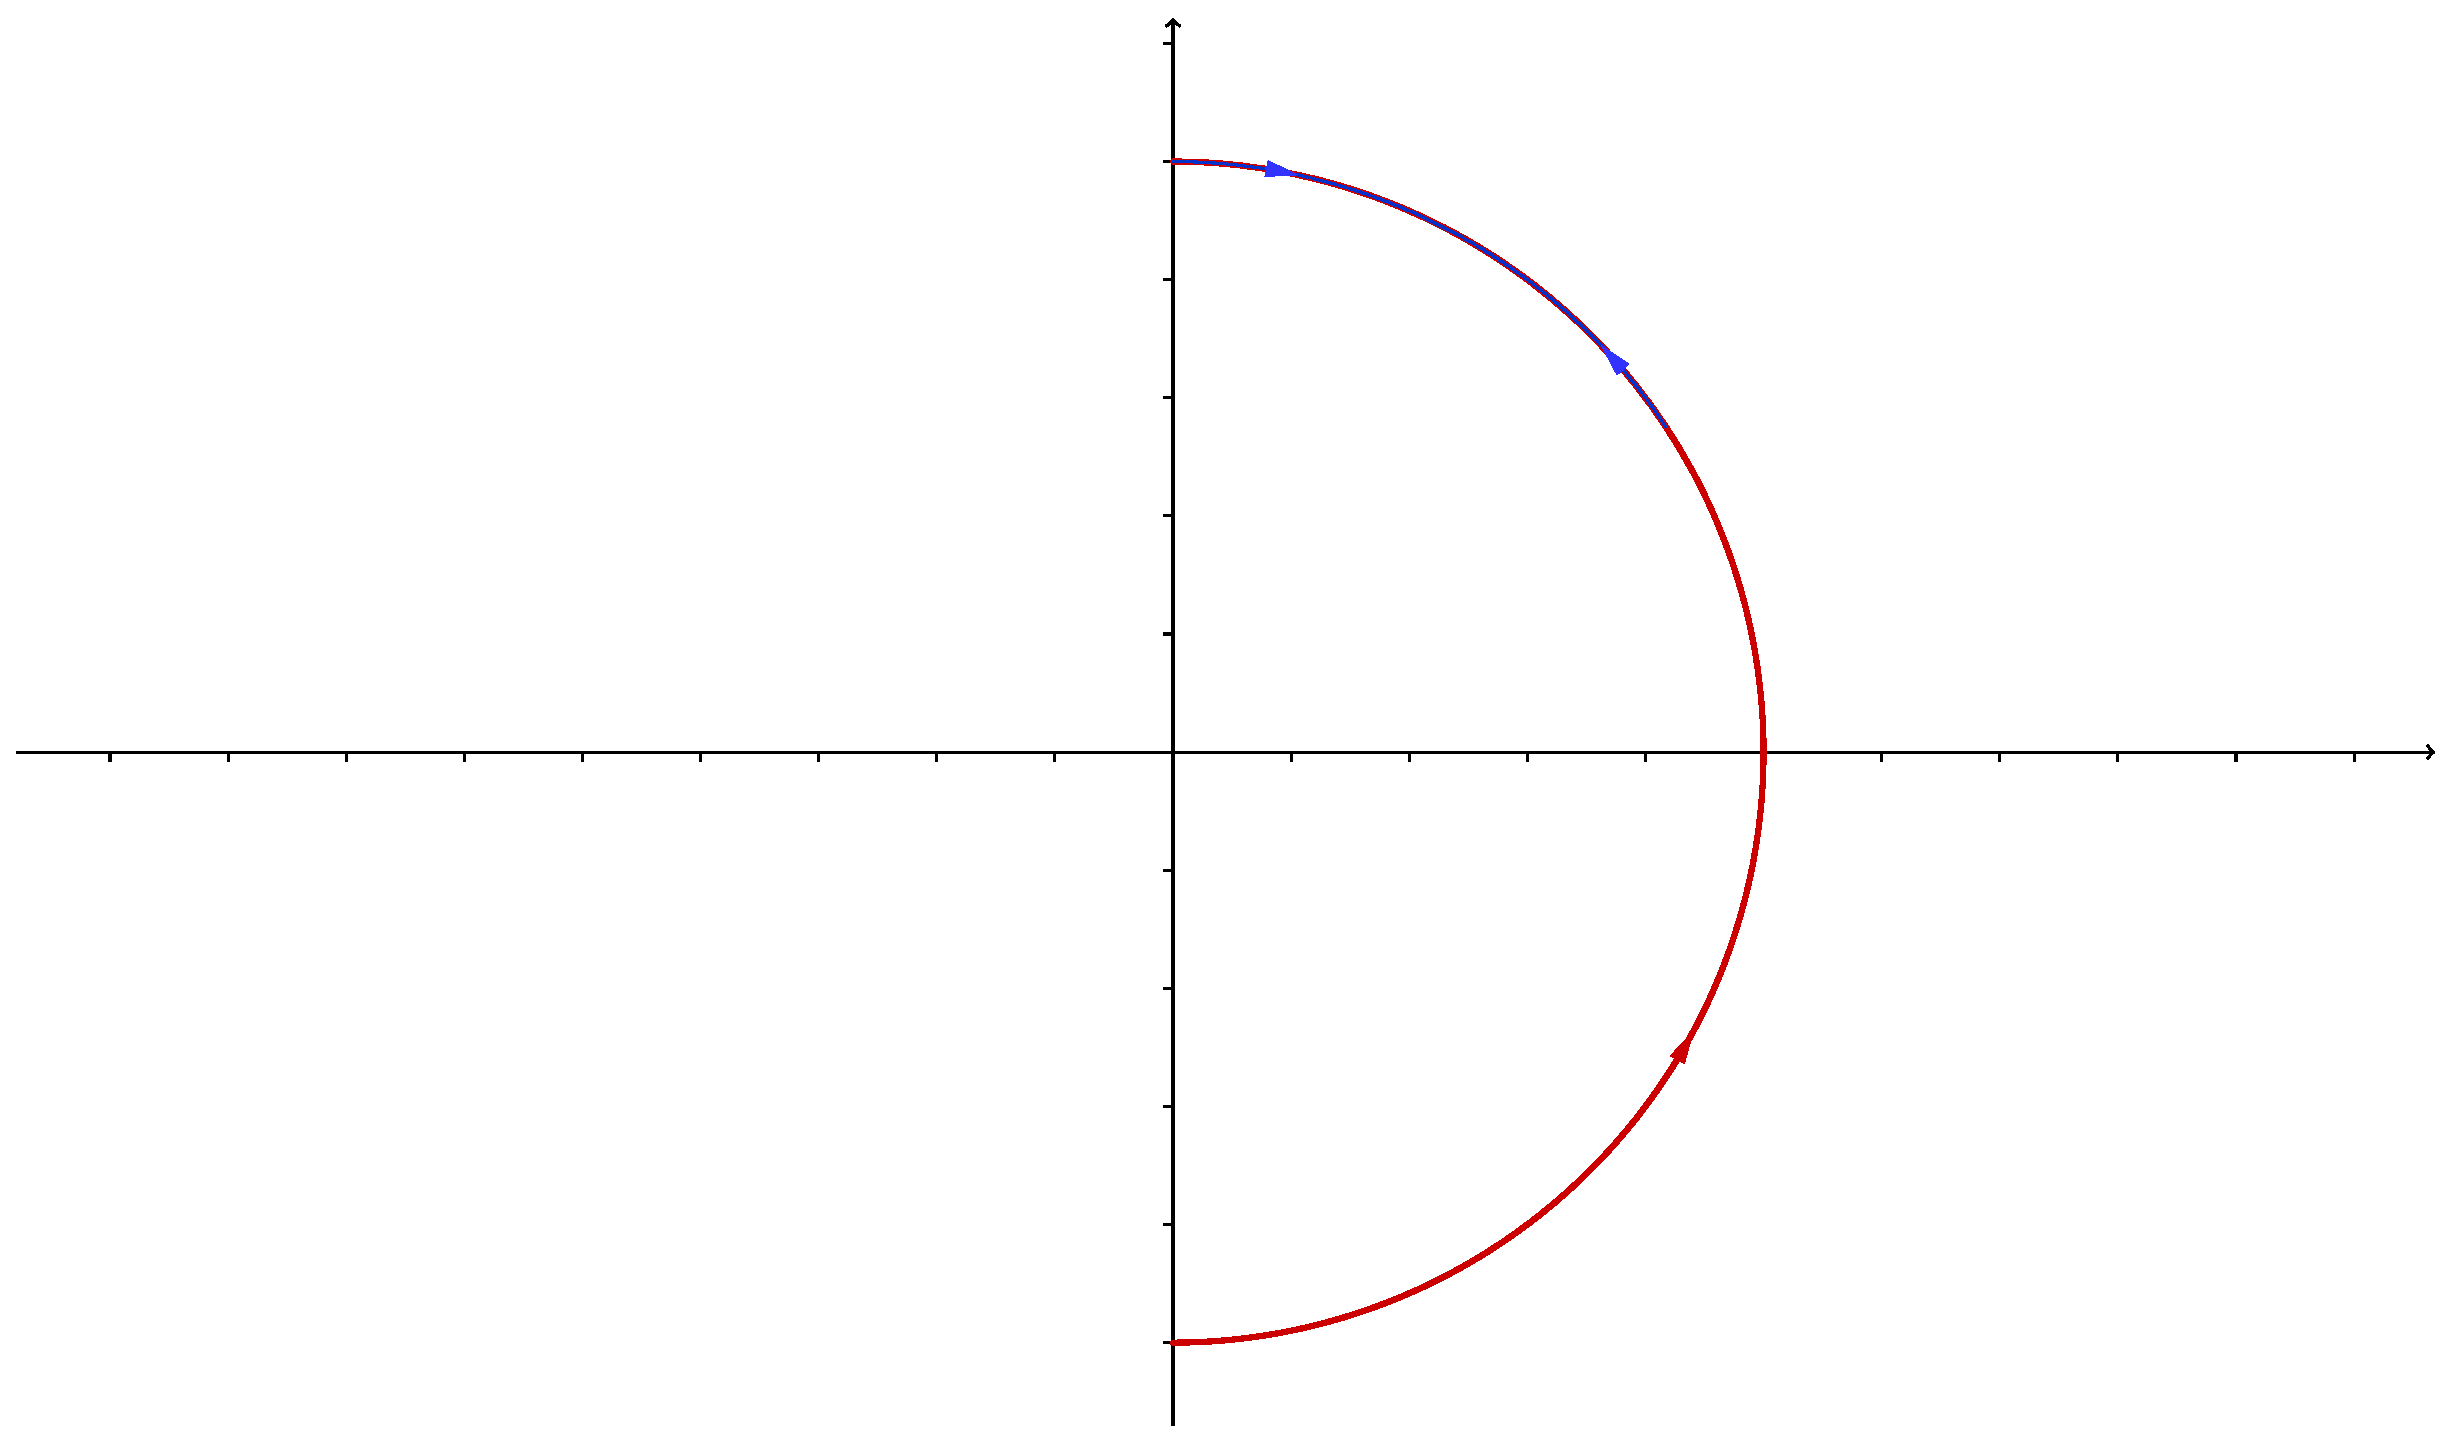
\includegraphics[width=0.5\textwidth]{Figures/Topologicalindex/topindex}  
\caption{In red (blue) $(h_x(k),h_z(k))$ is plotted as function of $k\in \{0, \infty\}$ for $\mu > 0$ ($\mu < 0$). Notice that for $\mu < 0$ the curve starts and ends at the north pole.}  
\label{fig.hhatplot}  
\end{center}    
\end{figure}

It is then clear, that as long as there is an energy gap, $\hat{h}(k)$ is well defined. Since $E_{F,k=0} = |\mu|$, we see that the energy is gapped exactly when $\mu \neq 0$. Finally, since $\Delta_{k=0} = 0$, we notice that: 
\begin{equation}
\hat{h}(k=0) = -\text{sgn}(\mu)\hat{z} = p_0\hat{z}, \hspace{0.5cm} \hat{h}(k=\infty) = \hat{z} = p_{\infty}\hat{z},
\label{eq.hhatk0kinfty}
\end{equation}
where $\text{sgn}$ denotes the sign function. The idea is then, that we can specify a number $\nu \in \{-1,1\}$ by:
\begin{equation}
\nu = p_0p_{\infty} = -\text{sgn}(\mu).
\label{eq.topinvnudefition}
\end{equation}
The claim is, that we have hereby defined a topological index, which specifies two states, that cannot be deformed into each other without closing the energy gap. Graphically this is clear from figure \ref{fig.hhatplot}. In red (blue) I have plotted the behaviour of $\hat{h}$ for $\mu > 0$ ($\mu < 0$), omitting the zero component $h_y$. For $\mu > 0$ we see, that we go from the south pole to the north pole as $k$ goes from $0$ to $\infty$. For $\mu < 0$ on the other hand, we see that $\hat{h}(k)$ starts out at the north pole, then goes somewhat along the circle arc before returning to the north pole. This is of course the same behaviour as written in equation \eqref{eq.hhatk0kinfty}. It is then clear, that there is no way of continuously deforming one map to the other. Further, we notice that the mapping becomes ill-defined exactly when $\mu = 0$. This is also evident from the appearance of $\text{sgn}(\mu)$ in $\nu$. We notice, that since $\mu(T) \to -\infty$ and $\Delta_k(T)\to 0$ for $T\to \infty$, the $\mu < 0$ phase is connected continously to the normal phase. Hence, the normal phase, and thereby also the vacuum, is associated with $\nu = 1$. 

For $T = 0$ the normal phase has $\mu = \epsilon_{F,0} > 0$. We can hereby distinguish between two regimes. The first is the weak coupling regime. The pairing does not significantly alter the chemical potential: $\mu(T=0) > 0$. Hereby $\nu = -1$ and the ground state is topologically \textit{non}-trivial. The second is the strong coupling regime, where $\mu(T = 0) < 0$, $\nu = 1$ and the ground state is topologically trivial. This is in complete harmony with the findings in \cite{Alicea} for the Kitaev chain.\footnote{In the article by Alicea the fermions sit in a lattice, but the physical properties are essentially the same.}

We are only investigating the weak coupling regime, even with $\mu \approx \epsilon_{F,0}$. From the above arguments, this means, that we have found a ground state with $\nu = -1$. So far, we have investigated the bulk properties of the superfluid by imposing cyclic boundary conditions. Imagine it now as a wire with open ends. This means, that there are junctions at the ends between a $\nu = -1$ (the superfluid wire) and a $\nu = 1$ state (the vacuum). It also means, that when we spatially follow the transition between the two phases, the wire and the vacuum, $\nu$ has to change its value abrubtly at the boundary. Hence, the energy gap has to dramatically drop to $0$ at the boundary. 

The interesting question is now: are there states that are topologically protected? More precisely, we are asking, whether there exist low energy states, that can only be removed by breaking the symmetries of the system. The answer lies in the build in particle-hole symmetry of the Hamiltonian. As we saw in section \ref{sec.SymmetriesTRandPH} we have a particle-hole symmetry $\mathcal{C} = \sigma_1 K$, with $K$ being the complex conjugation operator. Hereby $\mathcal{C}\mathcal{H}_{FF,k} = -\mathcal{H}_{FF,-k}\mathcal{C}$. Let us assume, that we have a single particle energy solution in $k$: $\mathcal{H}_{FF,k}\ket{\psi_k} = E_k\ket{\psi_k}$. We hereby directly get:
\begin{equation}
E_k\mathcal{C}\ket{\psi_k} = \mathcal{C}\mathcal{H}_{FF,k}\ket{\psi_k} = -\mathcal{H}_{FF,-k}\mathcal{C}\ket{\psi_k} \Rightarrow \mathcal{H}_{FF,-k}\left(\mathcal{C}\ket{\psi_k}\right) = -E_k\left(\mathcal{C}\ket{\psi_k}\right).
\end{equation}
This shows, that if $\ket{\psi_k}$ has the energy $E_k$, then $\mathcal{C}\ket{\psi_k}$ has the energy $-E_k$. In other words for every positive energy solution there is also a negative one, as is shown to the left in figure \ref{fig.edgestates}. The bulk spectrum is here indicated by a solid line above the bulk gap $\min_k[E_{F,k}]$ and mirrored in $E = 0$. Now suppose that we introduce a perturbation, that respects the particle-hole symmetry. The energies therefore still come in plus/minus pairs, but apart from that the energies can change. Hence, we can perturb any low energy state with $E \neq 0 $ away. This is indicated in the figure by the black dots and arrows. However, the \textit{single} state at $E = 0$ remains exactly there, because if it moved either up or down, there would not be the plus/minus symmetry in the energies. This leads to an energy spectrum, which is \textit{robust} against symmetry-conserving perturbations with the continuum above the bulk gap and a \textit{single} zero energy edge state as indicated in figure \ref{fig.edgestates}. 

With no energy cost edge states at the ends of the wire can hereby emerge and are robust to symmetry-conserving perturbations. This phenomenon is known as the bulk-edge correspondence principle, since it connects bulk effects, $\nu = -1$, to an edge effect (the edge states). As is indicated to the right in figure \ref{fig.edgestates}, the state has to be localised on the boundaries. The reason is, that all bulk states are already occupied, and so a zero energy bulk state is not available. 

\begin{figure}
\center
\begin{tikzpicture}
\draw[|->, thick] (0, 0) -- (0,  2) node[above]{$E$};
\draw[-, thick]   (0, 0) -- (0, -2);
\node at (-0.4, 0) {$0$};

\draw[-, dashed] (0, 1)--(1, 1);
\draw[-, thick] (-0.1, 1)--(0.1, 1);
\node at (-1.17,1) {$\min_k[E_{F,k}]$};

\draw[-, dashed] (0, -1)--(1, -1);
\draw[-, thick] (-0.1, -1)--(0.1, -1);
\node at (-1.35,-1) {$-\min_k[E_{F,k}]$};

\draw[-, ultra thick] (1, 1)--(1, 2);
\draw[-, ultra thick] (1, -1)--(1, -2);
\node[red] at (1, 0) {\textbullet};

\node at (1, 0.5) {\textbullet};
\draw[->] (1, 0.5) --  (1,  1);
\node at (1, -0.5) {\textbullet};
\draw[->] (1, -0.5) -- (1, -1);

\draw[-, dashed] (0,0.01) --(1,0.01);

\node at (3, -0.4) {$0$};
\node at (8, -0.4) {$\mathcal{L}$};
\draw[|->, thick ] (3,0) -- (9,0) node[right]{$x$};

\draw[-, ultra thick ] (3,0) -- (8,0);
\draw[scale=0.5,domain=-1:1,smooth,variable=\x,red] plot ({\x + 6},{ 3 * exp{- 10 * \x*\x}});
\draw[scale=0.5,domain=-1:1,smooth,variable=\x,red] plot ({\x + 16},{ 3 * exp{- 10 * \x*\x}});
\end{tikzpicture}
\caption{To the left the energy spectrum is sketched. Because of the particle-hole symmetry, there is a negative energy state for every positive. There is a continuum of states above $\min_k[E_{F,k}]$ and below $-\min_k[E_{F,k}]$. At the boundary of the wire the gap closes, but the particle-hole symmetry only protects the single state at $E = 0$, indicated by the red dot. The corresponding wave function is sketched to the right.}
\label{fig.edgestates}
\end{figure}

We can now also clarify, what is meant by the term \textit{topological} superfluid. The above mentioned effects are called topological, because the classification with respect to the symmetries $T,C$ and $S$ is deeply connected to topology; specifically the study of manifolds. This is of abstract parameter spaces, and so the naming as such does not originate from the fact, that the edge states are located at specific places geometrically, as one might be led to believe.  

\section{The Chern-Simons invariant and the Wilson loop}
\label{sec.CS1}
In this section we calculate the Chern-Simons topological invariant of the system and in turn the gauge independent Wilson loop. It is based on the article \cite{Ryu.Topology}. We do not anticipate any breaking of time reversal symmetry. The topological index is therefore to be found in the integers, $\mathbb{Z}$. We will work with $\Delta_k$ real. The calculation in this section is more rigorous but also less intuitive than the one in the previous section.

The Chern-Simons invariant is generally a half integer: $\dots, -3/2, -1, -1/2, 0, 1/2, \dots$. The topological index, generally called the winding number, is twice the Chern-Simons invariant, hence an integer. This gives us the desired topological index in $\mathbb{Z}$. In one spatial dimension the Chern-Simons invariant is generally defined as:
\begin{equation}
\text{CS}_1 = \frac{i}{2\pi}\int_{\text{BZ}}dk \; \text{tr}\left[\mathcal{A}_k\right], \nonumber
\end{equation}
where BZ is short for the first Brillouin zone, and $\mathcal{A}_k$ is the socalled Berry connection. In the literature the Chern-Simons invariant is also referred to as the (total) polarisation. This naming has a physical reasoning in electronic topological insulators, because it is actually a measure of the charge polarisation as a consequence of the edge states \cite{FuKane2006}. Since there are no charge carriers in our system, we will not use this naming. Now let $\ket{e^{-}_k}$ be the eigenvector to $\mathcal{H}_{FF,k}$ with eigenvalue $-E_{F,k}$. The Berry connection is then in this case defined as:
\begin{equation}
\mathcal{A}_k = \bra{e^{-}_k}\partial_k\ket{e^{-}_k}. \nonumber
\end{equation}
The result of Chern-Simons theory is then, that the Chern-Simons invariant is a topological invariant. By this, it is meant, that it characterizes different topological phases, that can only change when the energy gap closes. It turns out that the calculation in this scenario is easier in a different basis, than the one we have been working in so far. Let us therefore shortly investigate the influence of basis on the Berry connection. In a different basis we have: $\tilde{\mathcal{H}}_{FF,k} = U\mathcal{H}_{FF,k}U^\dagger$, where $U$ is some unitary matrix not depending on $k$. If $\mathcal{H}_{FF,k}\ket{e^{-}_k} = -E_{F,k}\ket{e^{-}_k}$, the eigenvector in the new basis with negative eigenvalue is $\ket{\tilde{e}^{-}_k} = U\ket{e^{-}_k}$. The corresponding Berry connection is:
\begin{equation}
\tilde{\mathcal{A}}_k = \bra{\tilde{e}^{-}_k}\partial_k\ket{\tilde{e}^{-}_k} = \bra{e^{-}_k}U^\dagger\partial_k U\ket{e^{-}_k} = \bra{e^{-}_k}\partial_k\ket{e^{-}_k} = \mathcal{A}_k, \nonumber 
\end{equation}
whereby the Berry connection and hereby the Chern-Simons invariant is unaltered. This is of course very reasonable; a topological invariant should not depend on the chosen basis. We now make a specific choice for $U$:
\begin{equation}
U = \text{e}^{i\sigma_1 \frac{3\pi}{4}} = \frac{1}{\sqrt{2}}\left(-\mathbb{I} + i\sigma_1\right). \nonumber 
\end{equation}
This transformation amounts to letting $(\sigma_1, \sigma_2, \sigma_3) \overset{U}{\to} (\sigma_1, \sigma_3, -\sigma_2)$. Since $\mathcal{H}_{FF,k} = \Delta_k\sigma_1 + \varepsilon_k\sigma_3$, in the new basis we get: $\tilde{\mathcal{H}}_{FF,k} = U\mathcal{H}_{FF,k}U^\dagger = \Delta_k\sigma_1 - \varepsilon_k\sigma_2$. The reason for changing basis is, that the eigenvectors are simpler. Explicitly:
\begin{equation}
\ket{\tilde{e}^{-}_k} = \frac{1}{\sqrt{2}}\begin{bmatrix} -\frac{\Delta_k + i \varepsilon_k}{E_{F,k}} \\ 1 \end{bmatrix}. \nonumber 
\end{equation}
With this and a bit of calculating the Berry connection becomes:
\begin{equation}
\mathcal{A}_k = \bra{\tilde{e}^{-}_k}\partial_k\ket{\tilde{e}^{-}_k} = -\frac{i}{2E^2_{F,k}}(\varepsilon_k\partial_k\Delta_k - \Delta_k \partial_k \varepsilon_k). \nonumber 
\end{equation}
Since the Brillouin zone is simply the entire axis, $k\in (-\infty, \infty)$, we get:
\begin{equation}
\text{CS}_1 = \frac{i}{2\pi}\int_{\text{BZ}} dk\; \text{tr}\left[\mathcal{A}_k\right] = \frac{1}{4\pi}\int_{-\infty}^{\infty} dk \;  \frac{\varepsilon_k\partial_k\Delta_k - \Delta_k \partial_k \varepsilon_k}{\varepsilon^2_k + \Delta^2_k} = \frac{1}{2\pi}\int_0^\infty dk \; \frac{\varepsilon_k\partial_k\Delta_k - \Delta_k \partial_k \varepsilon_k}{\varepsilon^2_k + \Delta^2_k}, 
\label{eq.CSinv1}
\end{equation}
where the last equality stems from the fact, that the integrand is even. The integrand has a primitive given by $-\arctan\left(\frac{\varepsilon_k}{\Delta_k}\right)$. Hence, the above is directly calculable:
\begin{align}
\text{CS}_1 &= - \frac{1}{2\pi} \left. \arctan\left(\frac{\varepsilon_k}{\Delta_k}\right)\right|^\infty_0 \overset{(*)}{=} -\frac{\text{sgn}(\Delta_{k>0})}{2\pi}\left(\frac{\pi}{2} - \lim_{a\to 0^{+}}\arctan\left(\frac{-\mu}{a}\right) \right) \nonumber \\
& = \left\{ \begin{matrix} -\frac{\text{sgn}(\Delta_{k>0})}{2}, & \mu > 0, \\ 0, & \mu < 0. \end{matrix} \right. 
\label{eq.CSinv2}
\end{align}
By $\text{sgn}(\Delta_{k>0})$ we mean the sign of $\Delta_k$ for $k > 0$. Two effects lead to the equality $(*)$. Firstly, $\arctan(x) \to \pi/2$ for $x \to \infty$. $\text{sgn}(\Delta_{k>0})$ appears, since if $\Delta_k$ is negative for $k > 0$, the argument $\frac{\varepsilon_k}{\Delta_k}$ goes to $-\infty$ for $k \to \infty$. Secondly, since $\Delta_{k=0} = 0$ the evaluation in $k = 0$ can be performed by the written limit of $a \to 0^+$. This shows, that the Chern-Simons invariant is \textit{not} invariant under gauge transformations, e.g. $\Delta_k \to - \Delta_k$. Since the two nonzero Chern-Simons invariants are related by a gauge transformation, they are equivalent. To account for this, we compute the \textit{gauge independent} Wilson loop $W_1$. We get: 
\begin{equation}
W_1 = \text{e}^{2\pi i \text{CS}_1} = -\text{sgn}(\mu). 
\end{equation}
We have $\Delta_k = 0$ in the normal phase, which is the topologically trivial phase. It therefore follows from equation \eqref{eq.CSinv1}, that $\text{CS}_1 = 0$ and hence $W_1 = 1$ for the trivial phase. This means, that $W_1 = -1$ is the (only) topological (non-trivial) phase. We also see, that the condition is exactly the same as the one found in the previous section. It is however quite satisfying to see, that we can come to this result in a more rigorous manner, also not assuming any brokenness of the time reversal symmetry. The edge states analysis of the previous section is unaltered in the present context.  

\vspace{1cm}
The question now becomes the following. Is it possible to make a simple physical change of the system, that allows us to observe a topological phase transition? The proposal is to put in a \textit{second} wire parallel to the already studied. By doing this we get two kinds of interactions. The first is the \textit{intra}wire interaction, the interaction internally in each wire, which we have already studied in detail. The second is the \textit{inter}wire interaction, the interaction between the two wires. Further, we get an extra parameter, namely the distance $d$ between the wires. It will allow us to study the transition between intrawire and interwire dominated interactions, and further what effect the topology has on the transition. This is the subject of part III of this thesis. 

